\documentclass[11pt]{article}
% Shared preamble of the project's LaTeX notes: notes/*.tex and the documents in literature/.
% Project macros go at the end. A macro copied from a paper's source goes in the note that
% quotes it, between its \input of this file and \begin{document}.
\usepackage[a4paper,margin=25mm]{geometry}
\usepackage{amsmath,amssymb,mathtools,bm}
\usepackage{graphicx,booktabs,xltabular}
\usepackage{xcolor}
\usepackage{xspace}
\usepackage[numbers,sort&compress]{natbib}
\bibliographystyle{apsrev4-2} % prints the arXiv ID of each entry in refs.bib
\usepackage[colorlinks,allcolors=blue!60!black]{hyperref}
\usepackage[notref,notcite]{showkeys} % prints each \label in the margin, so a pointer by label is found in the PDF
\renewcommand*\showkeyslabelformat[1]{\normalfont\tiny\ttfamily#1}

% Ragged-right X column for tables with prose cells: bridges, the survey's term map.
\newcolumntype{L}{>{\raggedright\arraybackslash}X}

% Project macros, in the notation of CONVENTIONS.md.
\newcommand{\GeV}{\mathrm{GeV}}
\newcommand{\MeV}{\mathrm{MeV}}
\newcommand{\vep}{{\bm p}}
\newcommand{\vek}{{\bm k}}
\newcommand{\veq}{{\bm q}}
\newcommand{\ver}{{\bm r}}
\newcommand{\vex}{{\bm x}}
\newcommand{\veA}{{\bm A}}
\newcommand{\vetau}{{\bm \tau}}
\newcommand{\veL}{{\bm L}}
\newcommand{\veS}{{\bm S}}
\newcommand{\ven}{{\bm n}}
\newcommand{\veep}{{\bm \epsilon}}
\newcommand{\veepst}{{\bm \epsilon}^{\prime*}}
\newcommand{\bbnP}{[\bar{b}b]_1(nP)}
\newcommand{\bbarb}{[\bar{b}b]_1}
\newcommand{\psibb}{\Psi^{(\bar{b}b)}}
\newcommand{\Mbb}{M^{(\bar{b}b)}}
\newcommand{\X}{X(3872)}
\newcommand{\Xb}{X_b}
\newcommand{\VQQ}{V^{(\bar{b}b)}}
\newcommand{\VOME}{V^{\rm (OME)}}
\newcommand{\TOME}{T^{\rm (OME)}}
\newcommand{\BOchiEFT}{BO$\chi$EFT\xspace}
\newcommand{\cyan}[1]{\textcolor{cyan}{#1}}

\usepackage{tikz}
% File names in prose: typewriter, breakable at / . - like a URL.
\newcommand{\file}[1]{\nolinkurl{#1}}
\title{What we solve for the $X_{b2}$: the $2^{++}$ Lippmann--Schwinger equation continued through its cuts}
\author{}
\date{2026-11-03}
\begin{document}
\maketitle

\noindent Notation follows \file{CONVENTIONS.md} (entries ``Lippmann--Schwinger equation'', ``Energy origin and on-shell momentum'', ``Pole position and Riemann sheets'', ``Continuation to other sheets'', ``Continued angular moments'', ``Projected OME potential''), terms follow \file{GLOSSARY.md}. Energies $E$ are measured from $2m_{B^*}=10649.50$~MeV, with the isospin-limit masses $m_B=5279.52$, $m_{B^*}=5324.75$, $m_\pi=138.039$, $m_\eta=548$~MeV and $\Delta m=m_{B^*}-m_B=45.23$~MeV. Short names: $P=B$, $V=B^*$, so $VV$, $PV$, $PP$ are the $B^*\bar B^*$, $C$-even $B\bar B^*$ and $B\bar B$ channels. Nothing here assumes where the $X_{b2}$ pole is. This note states the problem; \file{notes/07-continued-lse.tex} (note~07, whose labels are quoted as \texttt{07:st:closed} and so on) fixes the method and recomputes the singular points it needs.

\paragraph{The problem in brief.}
We want the poles of the $2^{++}$ $T$-matrix near the $B^*\bar B^*$ threshold, above all the $X_{b2}$. The $T$-matrix solves the six-channel Lippmann--Schwinger equation (LSE)~\eqref{eq:lse}; a pole is an energy at which the homogeneous form of that equation has a solution. In $1^{++}$ every state lay below every two-meson threshold, at real energy, and the LSE with its loop momentum on the real axis found it as the zero of a real determinant. In $2^{++}$ the channels $B\bar B(^1D_2)$ and $B\bar B^*(^3D_2)$ open $90.46$ and $45.23$~MeV below $2m_{B^*}$. A state near $2m_{B^*}$ can decay into them, so its pole leaves the real axis for an unphysical Riemann sheet, behind the right-hand (unitarity) cuts of those channels. The LSE on the real axis does not reach that sheet at any complex energy (Sec.~\ref{sec:rhc}). To reach it, the LSE has to be continued analytically through those cuts, by deforming the loop-momentum path into the lower half plane (Sec.~\ref{sec:contour}). For a potential that is smooth in the loop momentum this would be routine. The one-meson exchange (OME) is not smooth: it has branch points in the loop momentum, the same ones that give the on-shell potential its left-hand cut, and in time-ordered perturbation theory (TOPT) it has three-body branch points. They decide
\begin{enumerate}
\item how the exchange has to be evaluated at complex momenta (Sec.~\ref{sec:both}),
\item which deformations of the path are allowed, and how deep a pole can be reached (Secs.~\ref{sec:both}--\ref{sec:external}),
\item where the pole condition itself is cut on the unphysical sheets (Sec.~\ref{sec:lhc}).
\end{enumerate}
Section~\ref{sec:task} lists what has to be built and checked.

\section{The equation}\label{sec:equation}

The six channels (\file{CONVENTIONS.md}, ``2++ channel basis and projectors'') have thresholds $\delta_\alpha$ and reduced masses $\mu_\alpha$:
\begin{center}
\begin{tabular}{clrr}
\toprule
$\alpha$ & channel & $\delta_\alpha$ [MeV] & $\mu_\alpha$ [MeV]\\
\midrule
1--4 & $B^*\bar B^*$: $^5S_2$, $^1D_2$, $^5D_2$, $^5G_2$ & $0$ & $2662.38$\\
5 & $B\bar B^*(^3D_2)$, $C$-even & $-45.23$ & $2651.02$\\
6 & $B\bar B(^1D_2)$ & $-90.46$ & $2639.76$\\
\bottomrule
\end{tabular}
\end{center}
Channel $\alpha$ has on-shell momentum $k_\alpha$, $k_\alpha^2=2\mu_\alpha(E-\delta_\alpha)$; channels 1--4 share $k_1$. The potential is
\begin{equation}\label{eq:V}
V_{\alpha'\alpha}(p',p;E)=\delta_{\alpha'1}\delta_{\alpha1}\Bigl[\sum_{n=1}^{N}f_n(p')\,\frac{g^2}{E-E^{(0)}_n-V_0}\,f_n(p)+C\Bigr]+V^{\rm(OME)}_{\alpha'\alpha}(p',p;E):
\end{equation}
$s$-channel exchange of $N$ bare $\chi_{b2}$ states and the contact term, both acting only in the $S$-wave channel, plus the full OME (\file{CONVENTIONS.md}, ``Separable s-channel and contact potential'', ``2++ bare--continuum vertex''). The bare energies $E^{(0)}_n+V_0$ in $2^{++}$ are not yet chosen (\file{NOTEBOOK.md}, Open questions, Bare $\chi_{b2}$ masses); nothing below depends on them. The exchange is
\begin{gather}
V^{\rm(OME)}_{\alpha'\alpha}(p',q;E)=\frac1{10}\frac{g_b^2}{4F_\pi^2}\sum_{m=0}^{4}\mathcal N^{(m)}_{\alpha'\alpha}(p',q)\,\Delta^{(\beta_1\beta_2)}_m,\label{eq:VOME}\\
\Delta^{(\beta_1\beta_2)}_m=\int_{-1}^{1}dx\,x^m\bigl[D_{\beta_1}+D_{\beta_2}\bigr],\qquad
D_\beta=\frac{1}{2s(s+\nu_\beta)},\nonumber
\end{gather}
with $s=\sqrt{m_\phi^2+p'^2+q^2-2p'qx}$ the energy of the exchanged meson and $\nu_\beta$ the energy of the intermediate heavy pair of time ordering $\beta$ minus the total energy $M=2m_{B^*}+E$; for example $\nu_1=-2\Delta m+(p'^2+q^2)/(2m_B)-E$ for the $B\bar B\phi$ ordering. The isoscalar combination is $3V(m_\pi)+\frac13V(m_\eta)$ (\file{CONVENTIONS.md}, ``Projected OME potential'', ``Reduced masses and TOPT energy offsets''); the 21 independent entries are derived in \file{notes/04-ome-2pp.md}. There is no $PP\phi$ vertex, so $V^{\rm(OME)}_{56}=V^{\rm(OME)}_{66}=0$. Through $\nu_\beta$ the exchange depends on $E$.

The LSE is (\file{CONVENTIONS.md}, ``Lippmann--Schwinger equation''; Ref.~\cite{Zhang:2026iyr}, v1, Eqs.~(86)--(87))
\begin{equation}\label{eq:lse}
T_{\alpha'\alpha}(p',p;E)=V_{\alpha'\alpha}(p',p;E)-\sum_{\alpha''=1}^{6}\int_0^\Lambda\frac{q^2dq}{2\pi^2}\;
\underbrace{V_{\alpha'\alpha''}(p',q;E)}_{\text{left-hand, three-body cuts}}\;
\underbrace{G_{\alpha''}(k,q)}_{\text{right-hand cuts}}\;
T_{\alpha''\alpha}(q,p;E),
\end{equation}
\begin{equation}\label{eq:G}
G_\alpha(k,q)=\Bigl[\frac{q^2}{2\mu_\alpha}+\delta_\alpha-E-i\epsilon\Bigr]^{-1}=\frac{2\mu_\alpha}{q^2-k_\alpha^2-i\epsilon},
\end{equation}
with the sharp cutoff $\Lambda=4$~GeV. The labels under~\eqref{eq:lse} say where each singularity of the problem lives. The propagator has poles at $q=\pm k_\alpha$; they make the thresholds and the right-hand cuts. The exchange has branch points in the momenta; they make its left-hand and three-body cuts (Sec.~\ref{sec:cuts}). The bare-state term has poles in $E$ only, because the form factors $f_n$ are entire functions of momentum (\file{CONVENTIONS.md}, ``Bare-state term off the real axis'').

\paragraph{Pole condition.}
$T$ has a pole at $E$ when the homogeneous equation
\begin{equation}\label{eq:hom}
\psi_{\alpha'}(p')=-\sum_{\alpha''}\int\frac{q^2dq}{2\pi^2}\,V_{\alpha'\alpha''}(p',q;E)\,G_{\alpha''}(k,q)\,\psi_{\alpha''}(q)
\end{equation}
has a nonzero solution. On a quadrature grid $\{q_j,w_j\}$, Eq.~\eqref{eq:lse} becomes $(1+V\mathcal G)T=V$, where $V$ is the matrix of $V_{\alpha'\alpha''}(q_i,q_j;E)$ and $\mathcal G$ the diagonal matrix of $w_jq_j^2G_{\alpha''}(k,q_j)/(2\pi^2)$. The pole condition is
\begin{equation}\label{eq:D}
D(E)\equiv\det\bigl[1+V(E)\,\mathcal G(E)\bigr]=0 .
\end{equation}
Ref.~\cite{Zhang:2026iyr} (v1, Eq.~(93)) writes the same condition with the separable part eliminated. Write $V=V^{\rm(OME)}+F\hat vF^{\rm T}$, with $F$ the columns $f_{i,\alpha}(q_j)=\delta_{\alpha1}f_i(q_j)$, $f_{N+1}\equiv1$, and $\hat v={\rm diag}(v_1,\dots,v_{N+1})$ of v1, Eqs.~(60)--(63). Factoring out $1+V^{\rm(OME)}\mathcal G$ and using $\det(1+AB)=\det(1+BA)$,
\begin{align}
1+V\mathcal G&=\bigl(1+V^{\rm(OME)}\mathcal G\bigr)\bigl[1+(1+V^{\rm(OME)}\mathcal G)^{-1}F\hat vF^{\rm T}\mathcal G\bigr],\nonumber\\
D&=D^{\rm(OME)}\det\bigl[1+\hat v\hat J\bigr]=D^{\rm(OME)}\,\det\hat v\,\det\bigl(\hat v^{-1}+\hat J\bigr),\label{eq:Dfactor}
\end{align}
where $D^{\rm(OME)}=\det(1+V^{\rm(OME)}\mathcal G)$ and
\begin{equation}\label{eq:J}
\hat J=F^{\rm T}\mathcal G\bigl(1+V^{\rm(OME)}\mathcal G\bigr)^{-1}F=F^{\rm T}\mathcal GF-F^{\rm T}\mathcal G\,T^{\rm(OME)}\mathcal GF,\qquad T^{\rm(OME)}=\bigl(1+V^{\rm(OME)}\mathcal G\bigr)^{-1}V^{\rm(OME)},
\end{equation}
is the discretised $\hat J$ of v1, Eq.~(92); the second form uses $(1+V^{\rm(OME)}\mathcal G)^{-1}=1-T^{\rm(OME)}\mathcal G$. Away from the bare energies, where $\det\hat v$ has poles, and from zeros of $D^{\rm(OME)}$, where $\hat J$ is singular, the zeros of $\det(\hat v^{-1}+\hat J)$ are the zeros of $D$. The path of the loop integral enters both forms only through $\mathcal G$, so everything said below about $D$ holds for $\det(\hat v^{-1}+\hat J)$.

\section{What the real-axis LSE gives, and why it was enough in \texorpdfstring{$1^{++}$}{1++}}\label{sec:realaxis}

For real $E$ below the lowest threshold, $E<-90.46$~MeV, every $G_\alpha(k,q)$ is real, positive and smooth on $0\le q\le\Lambda$, and the exchange kernel is real and smooth for real momenta (Sec.~\ref{sec:kernel}). $D(E)$ is then a real function, and a pole is a real root, bracketed by a sign change. This is how every $1^{++}$ state was found (v1, Eq.~(96)) and how the package locates poles: its bracket ``must lie below every continuum threshold'' (\file{code/HadronDynamics.jl/docs/BOCHIEFT.md}, ``Bound poles and normalization''). It sufficed because every $1^{++}$ state lies below the lowest $1^{++}$ threshold, $B\bar B^*$; $B\bar B$ cannot form $1^{++}$.

In $2^{++}$ the same method covers every state below $2m_B=10559.04$~MeV. The measured $\chi_{b2}(9912)$ and $\chi_{b2}(10269)$ lie far below it and $\chi_{b2}(10524)$ lies $35$~MeV below it; whether the corresponding compact-dominated model states do is part of the result, not an input.

The $X_{b2}$ is sought near $2m_{B^*}$, $90.46$~MeV above $2m_B$. Heavy-quark spin symmetry makes it the partner of the $X_b$, which lies $91.0$~MeV (baseline fit) or $1$~MeV (shallow-$X_b$ fit) below its own threshold. The $2^{++}$ thresholds are split by $45.23$ and $90.46$~MeV, which is not small on either scale, so the $X_{b2}$ may lie in any of the four regions of Fig.~\ref{fig:energy}. This is orientation, not a prediction (\file{NOTEBOOK.md}, Open questions, $X_{b2}$ position).

\begin{figure}[t]
\centering
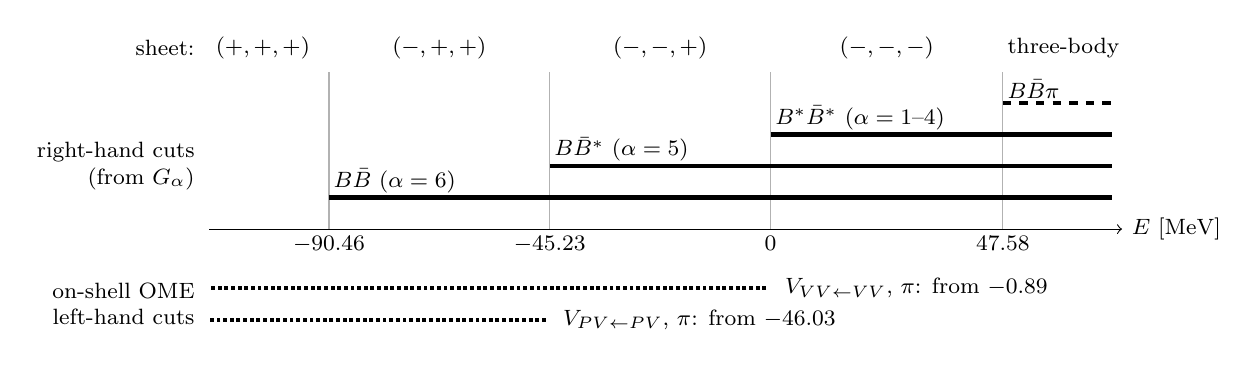
\begin{tikzpicture}[x=0.062cm,y=1cm,font=\footnotesize]
  % which sheet a pole is reported on, per region of Re E
  \node[anchor=east] at (-116,2.3) {sheet:};
  \node at (-104,2.3) {$(+,+,+)$};
  \node at (-67.85,2.3) {$(-,+,+)$};
  \node at (-22.62,2.3) {$(-,-,+)$};
  \node at (23.79,2.3) {$(-,-,-)$};
  \node at (60,2.3) {three-body};
  % threshold guides
  \foreach \e in {-90.46,-45.23,0,47.58} \draw[gray!60] (\e,0) -- (\e,2.0);
  % right-hand cuts
  \draw[line width=1.6pt] (-90.46,0.4) -- (70,0.4);
  \draw[line width=1.6pt] (-45.23,0.8) -- (70,0.8);
  \draw[line width=1.6pt] (0,1.2) -- (70,1.2);
  \draw[line width=1.6pt,dashed] (47.58,1.6) -- (70,1.6);
  \node[anchor=south west,inner sep=1.5pt] at (-90.46,0.4) {$B\bar B$ ($\alpha=6$)};
  \node[anchor=south west,inner sep=1.5pt] at (-45.23,0.8) {$B\bar B^*$ ($\alpha=5$)};
  \node[anchor=south west,inner sep=1.5pt] at (0,1.2) {$B^*\bar B^*$ ($\alpha=1$--$4$)};
  \node[anchor=south west,inner sep=1.5pt] at (47.58,1.6) {$B\bar B\pi$};
  \node[anchor=east,align=right] at (-116,0.8) {right-hand cuts\\(from $G_\alpha$)};
  % energy axis
  \draw[->] (-115,0) -- (72,0) node[right] {$E$ [MeV]};
  \node[anchor=north,fill=white,inner sep=1pt] at (-90.46,-0.05) {$-90.46$};
  \node[anchor=north,fill=white,inner sep=1pt] at (-45.23,-0.05) {$-45.23$};
  \node[anchor=north,fill=white,inner sep=1pt] at (0,-0.05) {$0$};
  \node[anchor=north,fill=white,inner sep=1pt] at (47.58,-0.05) {$47.58$};
  % on-shell left-hand cuts
  \draw[line width=1.4pt,densely dotted] (-0.89,-0.75) -- (-115,-0.75);
  \node[anchor=west] at (1,-0.75) {$V_{VV\leftarrow VV}$, $\pi$: from $-0.89$};
  \draw[line width=1.4pt,densely dotted] (-46.03,-1.15) -- (-115,-1.15);
  \node[anchor=west] at (-44.5,-1.15) {$V_{PV\leftarrow PV}$, $\pi$: from $-46.03$};
  \node[anchor=east,align=right] at (-116,-0.95) {on-shell OME\\left-hand cuts};
\end{tikzpicture}
\caption{The energy axis near $2m_{B^*}$. Top row: the sheet on which a pole whose $M$ lies in that region is reported; only the leftmost region is reached by the LSE on the real axis. Solid bars: two-body right-hand cuts, each starting at its threshold; dashed: the $B\bar B\pi$ three-body cut of the TOPT exchange. Dotted, below: the nearest left-hand cuts of the on-shell exchange (Table~\ref{tab:lhc}); the $VV$ pion cut starts $0.89$~MeV below $2m_{B^*}$, too close to resolve at this scale. They are cuts of on-shell matrix elements, not of the physical-sheet pole condition (Sec.~\ref{sec:lhc}). Sheet labels as in \file{CONVENTIONS.md}, ``Pole position and Riemann sheets''.}
\label{fig:energy}
\end{figure}

\section{Why the \texorpdfstring{$X_{b2}$}{Xb2} pole is out of reach: the right-hand cuts}\label{sec:rhc}

Take one channel and a factor $h(q)$ that is smooth near the real axis, and look at a single loop,
\begin{equation}\label{eq:loop}
I_\alpha(E)=\int_0^\Lambda\frac{q^2dq}{2\pi^2}\,\frac{2\mu_\alpha\,h(q)}{q^2-k_\alpha^2}.
\end{equation}
It is analytic in $E$ except where the pole $q=k_\alpha$ lands on the path: for real $E$ with $0<k_\alpha<\Lambda$, that is $\delta_\alpha<E<\delta_\alpha+\Lambda^2/(2\mu_\alpha)$. There the two sides differ. With $1/(x\mp i0)=\mathrm P(1/x)\pm i\pi\delta(x)$ and $\delta(q^2-k_\alpha^2)=\delta(q-k_\alpha)/(2k_\alpha)$,
\begin{equation}\label{eq:jump}
I_\alpha(E\pm i0)=\mathrm P\!\!\int_0^\Lambda\frac{q^2dq}{2\pi^2}\,\frac{2\mu_\alpha h(q)}{q^2-k_\alpha^2}\;\pm\;i\rho_\alpha h(k_\alpha),\qquad \rho_\alpha=\frac{\mu_\alpha k_\alpha}{2\pi}.
\end{equation}
$I_\alpha$ jumps by $2i\rho_\alpha h(k_\alpha)$ across the real axis, from the threshold on. Every loop in the LSE carries this jump, and so do $D$ and $T$: these are the right-hand cuts. The $-i\epsilon$ in~\eqref{eq:G} makes the upper rim, $T(E+i0)$, the physical amplitude; the sign $+i\rho_\alpha$ there is the $\operatorname{Im}T^{-1}=\rho$ of \file{CONVENTIONS.md}, ``Multichannel S matrix and unitarity''.

The LSE with $\int_0^\Lambda$ at complex $E$ defines one analytic function on the energy plane cut along these intervals (and, above $+47.58$~MeV, along the three-body cut): the physical sheet $(+,+,+)$. Its values with $\operatorname{Im}E<0$ join continuously onto the lower rim, $T(E-i0)$, not onto the physical amplitude. Continuing $T(E+i0)$ itself downward through the cut gives a different function, the physical-sheet one plus the jump (Sec.~\ref{sec:contour}): an unphysical sheet.

A state that can decay into an open channel produces a structure of width $\Gamma$ in $T(E+i0)$. Its pole is at $E_{\rm pole}=M-2m_{B^*}-i\Gamma/2$ on the sheet reached by continuing downward from the real segment that contains $M$; sheets are labelled by the signs of $\operatorname{Im}k$ at $B\bar B$, $B\bar B^*$, $B^*\bar B^*$ (\file{CONVENTIONS.md}, ``Pole position and Riemann sheets''):
\begin{center}
\begin{tabular}{rll}
\toprule
$M-2m_{B^*}$ [MeV] & open channels & sheet of a pole there\\
\midrule
below $-90.46$ & none & $(+,+,+)$, real $E$: a bound state\\
$-90.46$ to $-45.23$ & $B\bar B$ & $(-,+,+)$\\
$-45.23$ to $0$ & $B\bar B$, $B\bar B^*$ & $(-,-,+)$\\
$0$ to $47.58$ & all three & $(-,-,-)$\\
\bottomrule
\end{tabular}
\end{center}
A virtual state with respect to $B^*\bar B^*$, a pole below $2m_{B^*}$ with the $B^*\bar B^*$ sign flipped, lies on $(-,-,-)$ below its threshold, not on the sheet listed for its region. Above $+47.58$~MeV, where $B\bar B\pi$ opens, the three two-body signs no longer label all sheets.

Only the first row is accessible to the LSE on the real axis. This is the basic problem: unless the $X_{b2}$ lies below $2m_B$, its pole is on a sheet that the present solver does not compute.

\section{Reaching the other sheets: deforming the loop path}\label{sec:contour}

Replace $\int_0^\Lambda dq$ in~\eqref{eq:lse} by $\int_{\mathcal C}dq$ along a path $\mathcal C$ from $q=0$ to $q=\Lambda$ (\file{CONVENTIONS.md}, ``Continuation to other sheets''), and let $D_{\mathcal C}(E)$ be the corresponding determinant. Both ends are fixed: $q=0$ ends the radial integral and $q=\Lambda$ is the sharp cutoff. A rotation $q\to qe^{-i\theta}$ out to infinity, the usual complex scaling, is therefore not available; $\mathcal C$ leaves the real axis at $0$ and has to return to it at $\Lambda$.

\paragraph{Why this is the continuation.}
Let $\mathcal C$ run in $\operatorname{Re}q\ge0$, $\operatorname{Im}q\le0$. (i)~For $\operatorname{Im}E>0$ on the physical sheet, every $+k_\alpha$ lies in the upper half plane and every $-k_\alpha$ at $\operatorname{Re}q<0$, so deforming $[0,\Lambda]$ into $\mathcal C$ passes no propagator pole. If it moves no singularity of $V$ across the path either (Sec.~\ref{sec:both}), Cauchy's theorem, applied to each term of the Fredholm expansion of $D$, gives $D_{\mathcal C}(E)=D_{[0,\Lambda]}(E)$ there. (ii)~Now lower $E$ through the real axis above a threshold $\delta_\alpha$. The pole $+k_\alpha$ moves into the fourth quadrant. On $[0,\Lambda]$ it would hit the path, which is the cut; on $\mathcal C$ it does not, as long as it passes between $[0,\Lambda]$ and $\mathcal C$. So $D_{\mathcal C}$ stays analytic across the real axis: it is the continuation of the physical $D(E+i0)$, the sheet on which the sign of channel $\alpha$ is flipped. Which sheet is reached is fixed by which propagator poles lie between $[0,\Lambda]$ and $\mathcal C$ (Table~\ref{tab:paths}).
\begin{table}[h]
\centering
\begin{tabular}{lll}
\toprule
sheet & between $[0,\Lambda]$ and $\mathcal C$ & must stay outside (path passes above)\\
\midrule
$(-,+,+)$ & $+k_6$ & $-k_5$, $-k_1$\\
$(-,-,+)$ & $+k_5$, $+k_6$ & $-k_1$\\
$(-,-,-)$ & $+k_1$, $+k_5$, $+k_6$ & ---\\
\bottomrule
\end{tabular}
\caption{Propagator poles and the path, per sheet. Below its threshold with $\operatorname{Im}E<0$, an unflipped channel has $-k_\beta$ in the fourth quadrant near the negative imaginary axis; the path has to pass above it. On the physical sheet $\mathcal C=[0,\Lambda]$.}
\label{tab:paths}
\end{table}

\paragraph{The price, explicitly.}
The real segment followed by the reversed $\mathcal C$ encircles $+k_\alpha$ clockwise, so
\begin{align}
\int_{\mathcal C}\frac{q^2dq}{2\pi^2}G_\alpha(k,q)h(q)
&=\int_0^\Lambda\frac{q^2dq}{2\pi^2}G_\alpha(k,q)h(q)+2\pi i\operatorname*{Res}_{q=k_\alpha}\Bigl[\frac{q^2}{2\pi^2}\,\frac{2\mu_\alpha h(q)}{q^2-k_\alpha^2}\Bigr]\nonumber\\
&=\int_0^\Lambda\frac{q^2dq}{2\pi^2}G_\alpha(k,q)h(q)+2i\rho_\alpha h(k_\alpha),\label{eq:residue}
\end{align}
now with $k_\alpha$ in the lower half plane; the residue is $\mu_\alpha k_\alpha h(k_\alpha)/(2\pi^2)$. As $\operatorname{Im}E\to0^-$, Eq.~\eqref{eq:jump} turns the right-hand side into $I_\alpha(E-i0)+2i\rho_\alpha h(k_\alpha)=I_\alpha(E+i0)$: the path integral is continuous across the cut.

In the LSE the extra term is an insertion at the on-shell momentum. For one channel, write $G_{\mathcal C}=G_{[0,\Lambda]}+2i\rho\,|k\rangle\langle k|$ in the sense of~\eqref{eq:residue}, and let $T$ without subscript be the solution on $[0,\Lambda]$. Multiplying $(1+VG_{\mathcal C})T_{\mathcal C}=V$ by $(1+VG_{[0,\Lambda]})^{-1}$ gives $(1+2i\rho\,T|k\rangle\langle k|)\,T_{\mathcal C}=T$, a rank-one problem with solution
\begin{equation}\label{eq:onshellpoint}
T_{\mathcal C}(p',p)=T(p',p)-\frac{2i\rho\,T(p',k)\,T(k,p)}{1+2i\rho\,T(k,k)},\qquad
\frac{1}{T_{\mathcal C}(k,k)}=\frac{1}{T(k,k)}+2i\rho .
\end{equation}
Below the three-body threshold $T(E-i0)=T(E+i0)^*$ on the real axis, so $\operatorname{Im}T^{-1}(E-i0)=-\rho$ and $T_{\mathcal C}^{-1}(E-i0)=T^{-1}(E+i0)$: continuity again. The same steps for several channels, with $F$ the set of flipped channels, give for the determinant
\begin{equation}\label{eq:Dflip}
D_{\mathcal C}(E)=D_{[0,\Lambda]}(E)\,\det\nolimits_F\bigl[1+2i\rho_F\,T(k_F,k_F;E)\bigr].
\end{equation}
Eqs.~\eqref{eq:onshellpoint}--\eqref{eq:Dflip} are the on-shell-point route (\file{NOTEBOOK.md}, Decisions, Continuation route). They need $T(k_F,\cdot)$, the real-axis solution with one momentum at the complex on-shell value, and they need $T_{\mathcal C}(q,p)$ to be analytic in $q$ between the two paths. Section~\ref{sec:external} shows when either stops holding.

If $V$ were smooth in the loop momentum, this would be the whole story: any path obeying Table~\ref{tab:paths} gives the same $D_{\mathcal C}$, at any depth. The separable part of~\eqref{eq:V} is smooth in this sense. The exchange is not.

\section{The cut problem: what the one-meson exchange does}\label{sec:cuts}

\subsection{Where the exchange kernel is singular in the loop momentum}\label{sec:kernel}

The skeleton of every exchange entry is an $S$-wave static Yukawa exchange of mass $m$, used here only as an illustration, not as the model's OME:
\begin{equation}\label{eq:yukawa}
\int_{-1}^{1}\frac{dx}{m^2+p'^2+q^2-2p'qx}=\frac{1}{2p'q}\Bigl[\log\bigl(m^2+(p'+q)^2\bigr)-\log\bigl(m^2+(p'-q)^2\bigr)\Bigr].
\end{equation}
At fixed $p'$ it is singular where a logarithm's argument vanishes, at the four points $q=\pm p'\pm im$. Two consequences follow at once. In the loop momentum, for real $p'$, these points lie a distance $m$ above and below $\pm p'$, never on the real axis. On shell, $p'=q=k$, the right-hand side is $\frac{1}{2k^2}\log(1+4k^2/m^2)$, with a branch point at $k^2=-m^2/4$: the familiar left-hand cut. They are one set of singularities, seen once with $p'$ free and once with $p'$ tied to $E$.

The TOPT exchange~\eqref{eq:VOME} has the same structure with more points. After the angular integral its moments depend on $s_\pm=\sqrt{m_\phi^2+(p'\pm q)^2}$ and on $\log(s_\pm+\nu_\beta)$ (\file{CONVENTIONS.md}, ``Continued angular moments''; the moments are worked out in note~07, \texttt{07:st:closed}). In $q$, at fixed $p'$ and $E$, there are two kinds of branch points (\file{GLOSSARY.md}):
\begin{itemize}
\item \emph{exchanged-meson branch points}, $s_\pm=0$: $q=\pm p'\pm im_\phi$, as in~\eqref{eq:yukawa};
\item \emph{three-body branch points}, $s_\pm+\nu_\beta=0$: the intermediate three-body state $B^{(*)}\bar B^{(*)}\phi$ of ordering $\beta$ is on shell. With $\nu_1\simeq-2\Delta m-E$ at small momenta, the $B\bar B\pi$ points sit at $q\simeq\pm p'\pm i\sqrt{m_\pi^2-(2\Delta m+E)^2}$: $120$~MeV from $\pm p'$ at $E=-22.62$~MeV, $104$~MeV at $E=0$, and zero at the $B\bar B\pi$ threshold $E=m_\pi-2\Delta m=+47.58$~MeV. Keeping the $q^2$ term of $\nu_1$, the $p'=0$ points are at $q=\pm119.45\,i$ and $\pm103.38\,i$~MeV (\texttt{07:st:pzero}).
\end{itemize}
For real momenta neither kind is reached when $\operatorname{Re}E<47.58$~MeV: $s\ge m_\phi$, and $\operatorname{Re}(s+\nu_\beta)$, the heavy kinetic energies plus $s$ plus the heavy masses minus $\operatorname{Re}M$, is at least $E_{3,\beta}-\operatorname{Re}E>0$, where $E_{3,\beta}\ge47.58$~MeV is the three-body threshold of ordering $\beta$. So on $[0,\Lambda]$ the kernel is smooth in the momenta and analytic in $E$. This is why the $1^{++}$ calculation never met these singularities. Off the real axis they are what every deformation has to respect.

\subsection{The pole search: both momenta on the path}\label{sec:both}

In $D_{\mathcal C}$ both momenta of the kernel run on $\mathcal C$, so the exchanged-meson branch points move with the path: as $p'$ runs over $\mathcal C$ they sweep the curves $\mathcal C\pm im_\phi$ and $-\mathcal C\pm im_\phi$ (Fig.~\ref{fig:qplane}); the three-body branch points sweep curves close to $\mathcal C\pm i\sqrt{m_\phi^2-\nu_\beta^2}$. Let $\mathcal C$ be a graph path, $\operatorname{Re}q$ strictly increasing from $0$. Then $m_\phi^2+(p'-q)^2$ is zero or negative only if $p'-q$ is imaginary, i.e.\ $\operatorname{Re}p'=\operatorname{Re}q$, i.e.\ $p'=q$, where it equals $m_\phi^2$; and $m_\phi^2+(p'+q)^2$ only if $\operatorname{Re}(p'+q)=0$, i.e.\ $p'=q=0$. So along a graph path the exchanged-meson branch points never touch the path, and $s_\pm$ stay on their principal branches. The three-body branch points are not exact translates and have to be tested numerically; they close in on the path as $E$ approaches $+47.58$~MeV.

\paragraph{Consequence for resonance-type poles.}
For a pole on $(-,+,+)$, $(-,-,+)$ or $(-,-,-)$ with the flipped $+k_\alpha$ in the fourth quadrant away from the imaginary axis, a graph path obeying Table~\ref{tab:paths} exists, and the exchanged-meson branch points never cross it while it is deformed out of $[0,\Lambda]$. Whether the three-body branch points cross it is not settled here; the validator of note~07 (\texttt{07:st:validator}) tests it along the whole homotopy. Where the path passes, $D_{\mathcal C}$ on it is the continued pole condition (Sec.~\ref{sec:contour}; \texttt{07:st:continuation}), below the three-body threshold.

\paragraph{Admissibility.} \file{CONVENTIONS.md}, ``Continuation to other sheets'', calls a path admissible when a homotopy from $[0,\Lambda]$ at an energy with $\operatorname{Im}E_0>0$ reaches it while no propagator pole lies on the moving path and the kernel stays analytic with both momenta on it; that nothing lies between $[0,\Lambda]$ and $\mathcal C$ is required only of relations that compare the two paths at a fixed external momentum (Sec.~\ref{sec:external}). Once the path dips more than $m_\pi$ below the real axis, part of the swept curve $\mathcal C+im_\pi$ lies below the real axis, i.e.\ between $[0,\Lambda]$ and $\mathcal C$; the curve of three-body branch points, about $120$~MeV from the path near $E=-22.6$~MeV, gets there once the dip exceeds about $120$~MeV (Fig.~\ref{fig:qplane}b). Neither ever crosses $\mathcal C$, so neither bars such a path; the three-body branch points still have to be tested along the whole homotopy. The two conditions answer different questions. ``Nothing crosses'' is what Cauchy's theorem needs for $D_{\mathcal C}$ to be the continuation. ``Nothing lies between'' is what Eqs.~\eqref{eq:onshellpoint}--\eqref{eq:Dflip} need, since they compare the two paths one variable at a time with the other momentum held fixed. How deep a path has to go follows from $k_\alpha^2=2\mu_\alpha(E-\delta_\alpha)$: $\operatorname{Im}k_\alpha=\mu_\alpha\operatorname{Im}E/\operatorname{Re}k_\alpha$. At $\operatorname{Re}E=-22.62$~MeV on $(-,-,+)$, $|\operatorname{Im}k_5|$ reaches $119$~MeV at $\Gamma=33$~MeV and $m_\pi$ at $\Gamma=38.8$~MeV. A narrower pole is reached by a path shallow enough that nothing lies between the paths either (Fig.~\ref{fig:qplane}a).

\paragraph{Correct evaluation.}
What the exchange always demands is that it be evaluated on the right branch. At complex $p'$, $q$, $E$ the moments have to be built from separately continued $s_\pm$ and $L^{(\beta)}_\pm=\log(s_\pm+\nu_\beta)$, with their windings tracked from the real starting point (\file{CONVENTIONS.md}, ``Continued angular moments''). The principal logarithm of the ratio $(s_++\nu_\beta)/(s_-+\nu_\beta)$ is a different function off the real axis: it jumps along seams that are not singularities, and using it ``may lead to an incorrect result that breaks this analytic continuation'' (Ref.~\cite{Wu:2026wxb}, v1, App.~D, text after Eq.~(D1)).

\begin{figure}[p]
\centering
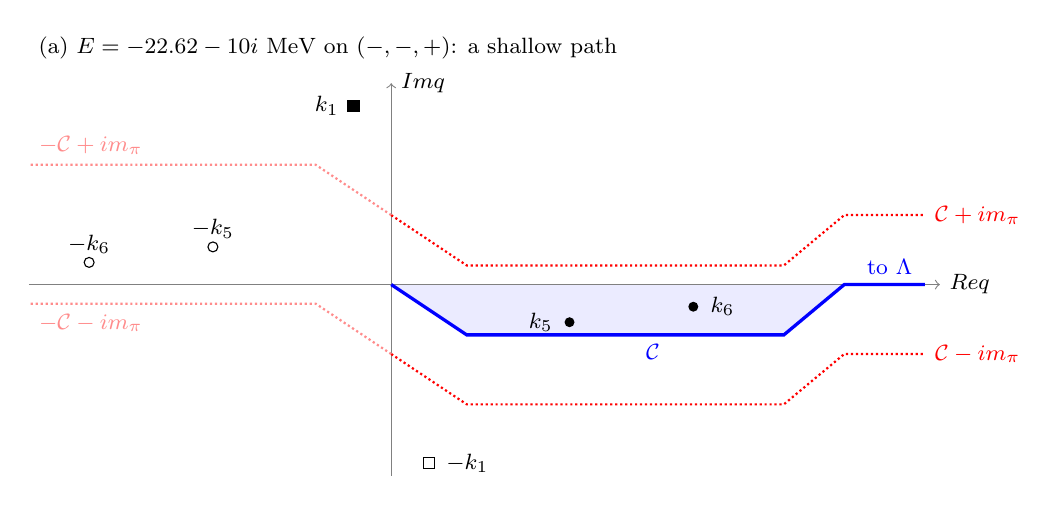
\begin{tikzpicture}[x=0.0064cm,y=0.0064cm,font=\footnotesize]
  \node[anchor=west] at (-720,470) {(a) $E=-22.62-10i$~MeV on $(-,-,+)$: a shallow path};
  \fill[blue!8] (0,0) -- (150,-100) -- (780,-100) -- (900,0) -- cycle;
  \draw[->,gray] (-720,0) -- (1090,0) node[right,black] {$\operatorname{Re}q$};
  \draw[->,gray] (0,-380) -- (0,400) node[right,black] {$\operatorname{Im}q$};
  % exchanged-meson branch points, swept as p' runs over C
  \draw[red,densely dotted,thick] (0,138) -- (150,38) -- (780,38) -- (900,138) -- (1060,138) node[right] {$\mathcal C+im_\pi$};
  \draw[red,densely dotted,thick] (0,-138) -- (150,-238) -- (780,-238) -- (900,-138) -- (1060,-138) node[right] {$\mathcal C-im_\pi$};
  \draw[red!45,densely dotted,thick] (0,138) -- (-150,238) -- (-720,238) node[above right] {$-\mathcal C+im_\pi$};
  \draw[red!45,densely dotted,thick] (0,-138) -- (-150,-38) -- (-720,-38) node[below right] {$-\mathcal C-im_\pi$};
  % path
  \draw[blue,very thick] (0,0) -- (150,-100) -- (780,-100) -- (900,0) -- (1060,0);
  \node[blue,anchor=north] at (520,-100) {$\mathcal C$};
  \node[blue,anchor=south] at (990,0) {to $\Lambda$};
  % propagator poles: filled = root on this sheet, open = its negative
  \fill (354.2,-74.8) circle[radius=1.8pt];
  \node[anchor=east] at (340,-74.8) {$k_5$};
  \fill (600.1,-44.0) circle[radius=1.8pt];
  \node[anchor=west] at (615,-44.0) {$k_6$};
  \draw (-354.2,74.8) circle[radius=1.8pt] node[anchor=south,inner sep=3pt] {$-k_5$};
  \draw (-600.1,44.0) circle[radius=1.8pt] node[anchor=south,inner sep=3pt] {$-k_6$};
  \filldraw (-75.0,355.1) +(-2pt,-2pt) rectangle +(2pt,2pt);
  \node[anchor=east] at (-85,355.1) {$k_1$};
  \draw (75.0,-355.1) +(-2pt,-2pt) rectangle +(2pt,2pt);
  \node[anchor=west] at (90,-355.1) {$-k_1$};
\end{tikzpicture}

\vspace{4mm}
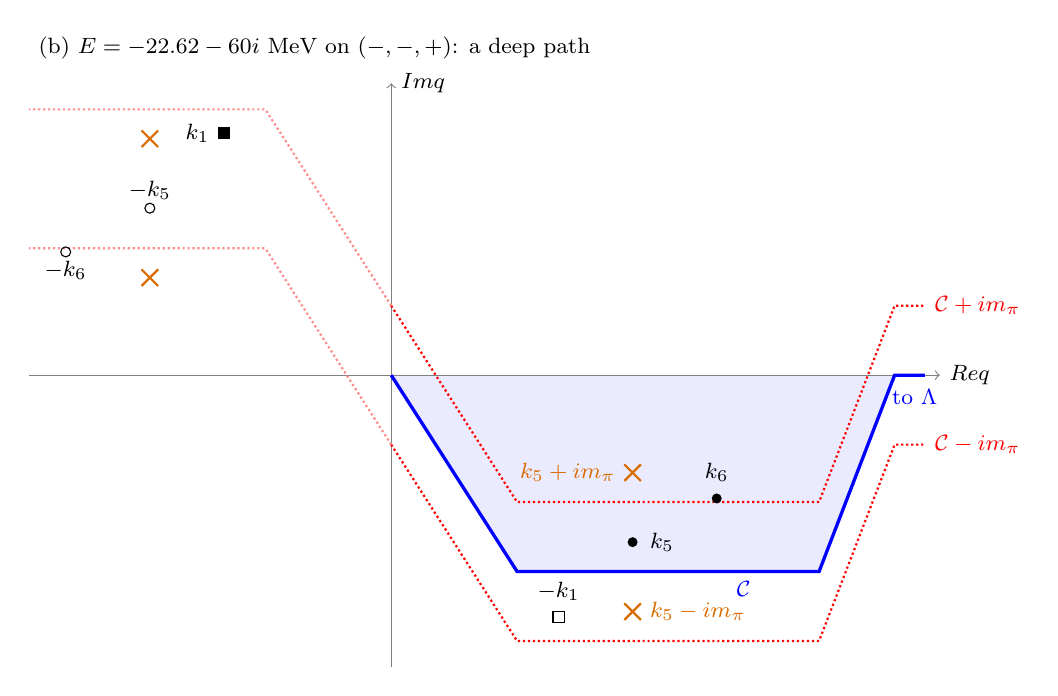
\begin{tikzpicture}[x=0.0064cm,y=0.0064cm,font=\footnotesize]
  \node[anchor=west] at (-720,650) {(b) $E=-22.62-60i$~MeV on $(-,-,+)$: a deep path};
  \fill[blue!8] (0,0) -- (250,-390) -- (850,-390) -- (1000,0) -- cycle;
  \draw[->,gray] (-720,0) -- (1090,0) node[right,black] {$\operatorname{Re}q$};
  \draw[->,gray] (0,-580) -- (0,580) node[right,black] {$\operatorname{Im}q$};
  % exchanged-meson branch points, swept as p' runs over C
  \draw[red,densely dotted,thick] (0,138) -- (250,-252) -- (850,-252) -- (1000,138) -- (1060,138) node[right] {$\mathcal C+im_\pi$};
  \draw[red,densely dotted,thick] (0,-138) -- (250,-528) -- (850,-528) -- (1000,-138) -- (1060,-138) node[right] {$\mathcal C-im_\pi$};
  \draw[red!45,densely dotted,thick] (0,138) -- (-250,528) -- (-720,528);
  \draw[red!45,densely dotted,thick] (0,-138) -- (-250,252) -- (-720,252);
  % path
  \draw[blue,very thick] (0,0) -- (250,-390) -- (850,-390) -- (1000,0) -- (1060,0);
  \node[blue,anchor=north] at (700,-390) {$\mathcal C$};
  \node[blue,anchor=north] at (1040,-8) {to $\Lambda$};
  % propagator poles
  \fill (479.5,-331.7) circle[radius=1.8pt];
  \node[anchor=west] at (495,-331.7) {$k_5$};
  \fill (646.6,-244.9) circle[radius=1.8pt];
  \node[anchor=south] at (646.6,-230) {$k_6$};
  \draw (-479.5,331.7) circle[radius=1.8pt] node[anchor=south,inner sep=3pt] {$-k_5$};
  \draw (-646.6,244.9) circle[radius=1.8pt] node[anchor=north,inner sep=3pt] {$-k_6$};
  \filldraw (-332.4,480.6) +(-2pt,-2pt) rectangle +(2pt,2pt);
  \node[anchor=east] at (-342,480.6) {$k_1$};
  \draw (332.4,-480.6) +(-2pt,-2pt) rectangle +(2pt,2pt);
  \node[anchor=south] at (332.4,-468) {$-k_1$};
  % exchanged-meson branch points of V(k_5,q), external momentum fixed at k_5
  \foreach \x/\y in {479.5/-193.7, 479.5/-469.8, -479.5/469.7, -479.5/193.7}
    \draw[thick,orange!85!black] (\x,\y) +(-3pt,-3pt) -- +(3pt,3pt) +(-3pt,3pt) -- +(3pt,-3pt);
  \node[anchor=east,orange!85!black] at (465,-193.7) {$k_5+im_\pi$};
  \node[anchor=west,orange!85!black] at (495,-469.8) {$k_5-im_\pi$};
\end{tikzpicture}
\caption{The loop-momentum plane at two probe energies on $(-,-,+)$, not predicted poles; coordinates in MeV. Thick: the path $\mathcal C$, which runs on along the real axis to $\Lambda=4$~GeV; shaded: the region between $[0,\Lambda]$ and $\mathcal C$. Circles: $\pm k_5$, $\pm k_6$; squares: $\pm k_1$; filled: the root on this sheet, open: its negative. The path passes below the flipped $k_5$, $k_6$ and above the unflipped $-k_1$ (Table~\ref{tab:paths}). Dotted: the curves swept by the exchanged-meson branch points of the kernel as $p'$ runs over $\mathcal C$ (Sec.~\ref{sec:both}); the three-body branch points, not drawn, lie about $120$~MeV from $\mathcal C$ at this $\operatorname{Re}E$. Crosses in (b): the exchanged-meson branch points of the half-off-shell kernel $V(k_5,q)$, with the external momentum fixed at $k_5$ (Sec.~\ref{sec:external}). In (a), $|\operatorname{Im}k_5|=75$~MeV and nothing but $k_5$, $k_6$ lies between the paths. In (b), $|\operatorname{Im}k_5|=332$~MeV: part of $\mathcal C+im_\pi$ and the point $k_5+im_\pi$ lie between the paths, although neither crosses $\mathcal C$ while it is deformed; the point $k_5-im_\pi$ is crossed if $[0,\Lambda]$ is deformed into this path before the energy is lowered (Sec.~\ref{sec:external}).}
\label{fig:qplane}
\end{figure}

\subsection{Fixed external momenta: on-shell amplitudes, couplings, the on-shell-point route}\label{sec:external}

Anything evaluated at an on-shell momentum contains the half-off-shell kernel $V(k_{\alpha'},q;E)$ with $k_{\alpha'}$ fixed: $T$ on shell at complex $E$, the couplings $g_\alpha$ of \file{CONVENTIONS.md}, ``Resonance couplings'', and Eqs.~\eqref{eq:onshellpoint}--\eqref{eq:Dflip}. Its exchanged-meson branch points are the fixed points $q=\pm k_{\alpha'}\pm im_\phi$, and its three-body branch points behave likewise. For a flipped channel $k_{\alpha'}=a-ib$ lies in the fourth quadrant; the point $k_{\alpha'}+im_\phi=a+i(m_\phi-b)$ is above the real axis while $b<m_\phi$, and crosses $[0,\Lambda]$ at $q=a$ when $b=m_\phi$. Beyond that:
\begin{itemize}
\item The real-axis $T(k_{\alpha'},\cdot)$ is no longer the continued function. The integral along $[0,\Lambda]$ has to be supplemented by the discontinuity along the cut from that point, and ``the result will be incorrect if this piece is ignored'' (Ref.~\cite{Wu:2026wxb}, v1, App.~D, contour $C_R'$ of Fig.~11). Eqs.~\eqref{eq:onshellpoint}--\eqref{eq:Dflip} therefore hold as written only while no singularity of $V(k_F,q;E)$ lies between the two paths (\file{CONVENTIONS.md}, ``Continuation to other sheets''; \file{NOTEBOOK.md}, Decisions, Continuation route): $|\operatorname{Im}k_F|<m_\pi$ for the exchanged-meson branch points, and less for the three-body ones. For $PV\leftarrow PV$ the $B\bar B\pi$ ordering has $\nu_\beta\simeq-\Delta m$ at $p'=k_5$, $q\simeq k_5$, so $s_-+\nu_\beta=0$ at $q\simeq k_5\pm i\sqrt{m_\pi^2-\Delta m^2}=k_5\pm130.4\,i$~MeV, and the route ends near $|\operatorname{Im}k_5|=130$~MeV (derived, not checked).
\item The point lies between $[0,\Lambda]$ and every path that passes below $k_{\alpha'}$ (Fig.~\ref{fig:qplane}b), although it never crosses $\mathcal C$. The other point, $k_{\alpha'}-im_\phi$, is crossed by a path already deeper than $m_\phi$ at $\operatorname{Re}q\simeq\operatorname{Re}k_{\alpha'}$ before the energy is lowered: at $E_0=-22.62+i0$, $k_5=346.2$~MeV, and the deep path of Fig.~\ref{fig:qplane}b lies $390$~MeV below the real axis there, so deforming $[0,\Lambda]$ into it at $E_0$ crosses $q=346.2-138\,i$~MeV. An on-shell quantity on such a path therefore needs a path lowered together with $E$, its depth at $\operatorname{Re}k_{\alpha'}$ kept between $b$ and $b+m_\phi$, or the cut terms of the first item (derived, not checked).
\end{itemize}
The pole position from $D_{\mathcal C}$ involves no fixed external momentum and is not affected by these points; on-shell amplitudes and couplings of a broad state are.

\subsection{The on-shell left-hand cuts inside the pole condition}\label{sec:lhc}

Eq.~\eqref{eq:Dflip} shows where the on-shell left-hand cuts enter the pole condition. The first factor, the physical-sheet determinant, has none: its kernel is analytic in $E$ for real momenta (Sec.~\ref{sec:kernel}), and only putting momenta on shell creates the left-hand cut. This is why the $1^{++}$ poles, whose binding momenta lie beyond $\kappa_{\rm lhc}=65$~MeV (v1, Eq.~(9)), were found without trouble. The second factor carries the on-shell amplitude among the flipped channels, together with its left-hand cuts, at the flipped momenta. The nearest on-shell branch points at tree level are listed in Table~\ref{tab:lhc}.
\begin{table}[h]
\centering
\begin{tabular}{llll}
\toprule
transition & $\phi$ & branch point & $E_L$ [MeV]\\
\midrule
$VV\leftarrow VV$ & $\pi$ & $k_1^2=-m_\pi^2/4$ & $-m_\pi^2/(4m_{B^*})=-0.89$\\
$VV\leftarrow VV$ & $\eta$ & $k_1^2=-m_\eta^2/4$ & $-14.10$\\
$PV\leftarrow PV$ & $\pi$ & $k_5^2=-\frac14(m_\pi^2-\Delta m^2)$ & $-46.03$\\
$PP\leftarrow PP$, $PP\leftrightarrow PV$ & --- & no exchange & ---\\
\bottomrule
\end{tabular}
\caption{Nearest branch points of the on-shell exchange. For $VV\leftarrow VV$ the on-shell offsets of the two orderings vanish and the denominator is exactly of the Yukawa form~\eqref{eq:yukawa} with $m_\pi$; for $PV\leftarrow PV$ it is Yukawa with $m_\pi^2-\nu_{\rm on}^2$, $\nu_{\rm on}\simeq-\Delta m$, which is v1, Eq.~(8) ($\kappa_{\rm lhc}=65.21$~MeV). The inelastic $VV\leftrightarrow PV$ and $VV\leftrightarrow PP$ branch points are listed in note~07, \texttt{07:st:endpoints}; which sheets carry their cuts is not derived there.}
\label{tab:lhc}
\end{table}

What this means for the $X_{b2}$:
\begin{itemize}
\item \emph{Bound-state-like, on $(-,-,+)$} (flipped $F=\{5,6\}$). The nearest tree-level cut of $T_{FF}$ is the $PV\leftarrow PV$ pion cut below $E=-46.03$~MeV, under the $B\bar B^*$ threshold; $T_{56}$ and $T_{66}$ have no tree-level exchange. For $-45.23<\operatorname{Re}E<0$ the pole condition therefore has no tree-level left-hand cut, however deeply the $X_{b2}$ is bound with respect to $B^*\bar B^*$. In particular the $VV$ pion cut at $-0.89$~MeV does not enter, because $B^*\bar B^*$ is not flipped. Iterated exchange adds further singularities to $T_{FF}$; they are not yet located.
\item \emph{Virtual state, on $(-,-,-)$ below threshold.} $B^*\bar B^*$ is flipped and the $VV\leftarrow VV$ factor enters at the flipped $k_1$. The elastic on-shell potential depends on $k_1^2$ only, so its cut $k_1^2<-m_\pi^2/4$ appears on this sheet along $k_1=-i\kappa_1$, $\kappa_1>m_\pi/2=69.02$~MeV, below $E=-0.89$~MeV. That is where a virtual state sits. One with binding energy $E_B<0.89$~MeV is an ordinary zero of $D_{\mathcal C}$; a deeper one lies on a cut of the pole condition and has to be reported with a side.
\item \emph{The path meets the same cut.} To keep $+k_1\simeq-i\kappa_1$ between $[0,\Lambda]$ and $\mathcal C$ as $\operatorname{Im}E\to0$, the path is squeezed against the negative imaginary axis, where the reflected curves $-\mathcal C\pm im_\pi$ reach it. In the limiting geometry $p'=q=-i\kappa_1$, $E=-\kappa_1^2/m_{B^*}$, the $VV\leftarrow VV$ kernel has $s_+^2=m_\pi^2+(p'+q)^2=m_\pi^2-4\kappa_1^2$ and $\nu_2=(p'^2+q^2)/(2m_{B^*})-E=0$, so its exchanged-meson branch point is hit at $\kappa_1=m_\pi/2$: the path fails where the function it computes has its branch point. If one path serves all channels, the $PV\leftarrow PV$ kernel is evaluated there too; its $B\bar B\pi$ ordering has $\nu_1=-2\Delta m-\kappa_1^2(1/m_B-1/m_{B^*})$, and $s_++\nu_1=0$ gives $\kappa_1=52.13$~MeV ($E=-0.51$~MeV), close to $\frac12\sqrt{m_\pi^2-4\Delta m^2}$. One path per channel removes this earlier obstruction (\file{NOTEBOOK.md}, Open questions, One contour or one per channel).
\item \emph{Couplings.} A residue needs the on-shell $T$ at the pole on its sheet, so the on-shell cuts of all channels matter, not only the flipped ones. The $B^*\bar B^*$ coupling of a $(-,-,+)$ pole with $E_B>0.89$~MeV, for example, is evaluated beyond the $VV$ pion branch point and needs a stated side.
\end{itemize}
Eq.~\eqref{eq:Dflip} was derived above on the condition that no kernel singularity lies between the paths. Its multichannel TOPT form, the iterated cuts and admissibility throughout $(-,-,+)$ and $(-,-,-)$ are unchecked (\file{NOTEBOOK.md}, Open questions, Pole condition in full TOPT).

\subsection{The three-body threshold}\label{sec:threebody}

At $E=+47.58$~MeV the $B\bar B\pi$ state goes on shell inside the exchange: the three-body branch points reach the real axis and the physical-sheet kernel acquires its own cut. Beyond it the three two-body signs do not label all sheets, and the path prescription above does not say which three-body sheet is reached. Below it, the three-body branch points are the singularities nearest to the path on $(-,-,-)$ and limit how far a graph path reaches there (Sec.~\ref{sec:kernel}; \texttt{07:st:quartic}).

\section{What has to be solved}\label{sec:task}

In one line: compute $\det[\hat v^{-1}+\hat J_{\mathcal C}(E)]$, the pole condition~\eqref{eq:Dfactor} on a deformed path, and find its zeros on the sheet that matches $\operatorname{Re}E$. The pieces:
\begin{enumerate}
\item \emph{Continued kernel.} $V^{\rm(OME)}_{\alpha'\alpha}(p',q;E)$ at complex $p'$, $q$, $E$ from separately continued $s_\pm$ and $L^{(\beta)}_\pm$ with tracked windings (Sec.~\ref{sec:both}); $f_n(p)$ at complex $p$ as in \file{CONVENTIONS.md}, ``Bare-state term off the real axis'', with transposes in every loop sum.
\item \emph{Path.} For each target sheet, a path from $0$ to $\Lambda$ obeying Table~\ref{tab:paths}, a graph path for resonance-type poles, reached from $[0,\Lambda]$ by a homotopy that never puts a propagator pole or a kernel singularity on it (\file{CONVENTIONS.md}, ``Continuation to other sheets''). Its quadrature nodes and weights are complex.
\item \emph{Continued two-potential solution.} The OME-only LSE (v1, Eq.~(88)) solved on $\mathcal C$, then $\hat J_{\mathcal C}$ from v1, Eq.~(92), or~\eqref{eq:J}, with $\int_0^\Lambda\to\int_{\mathcal C}$. The parameters $C$ and $V_0$ enter only through $\hat v$, as in $1^{++}$.
\item \emph{Pole search.} Zeros of $\det(\hat v^{-1}+\hat J_{\mathcal C})$ with $\operatorname{Re}E<47.58$~MeV on $(-,+,+)$, $(-,-,+)$, $(-,-,-)$, counted by the argument principle on closed curves free of branch points, then refined. States below $2m_B$ come from $\mathcal C=[0,\Lambda]$, as now.
\item \emph{Validation before any pole counts}, chosen on 2026-11-04 (\file{NOTEBOOK.md}, Decisions, Checks per stage):
\begin{enumerate}
\item Continuity: as $\operatorname{Im}E\to0^-$ on the adjacent sheet, the on-shell $T$ computed on $\mathcal C$ tends to the real-axis $T(E+i0)$, and $\operatorname{Im}T^{-1}=\rho$ holds there.
\item Path independence: $D_{\mathcal C}$ unchanged under admissible deformations of $\mathcal C$, including a shallow against a deep path at a narrow probe energy.
\item $\mathcal C=[0,\Lambda]$ and a deformed physical-sheet path reproduce the $1^{++}$ bound states of both fits.
\item Second route: Eqs.~\eqref{eq:onshellpoint}--\eqref{eq:Dflip} where nothing lies between the paths (Sec.~\ref{sec:external}).
\item A rank-one separable model with the three $2^{++}$ thresholds, solvable in closed form on every sheet, against the path solver.
\item Factorisation: $D_{\mathcal C}$ against $D^{\rm(OME)}_{\mathcal C}\det(1+\hat v\hat J_{\mathcal C})$ away from the bare energies and the zeros of $D^{\rm(OME)}$.
\end{enumerate}
\end{enumerate}

\paragraph{Where the method stops.}
A virtual state with respect to $B^*\bar B^*$ deeper than $\kappa_1=69.02$~MeV ($52.13$~MeV with one common path); $\operatorname{Re}E\ge47.58$~MeV; on-shell amplitudes and couplings beyond the on-shell branch points, or on paths whose homotopy crosses a singularity of the half-off-shell kernel (Sec.~\ref{sec:external}); and poles for which no admissible graph path exists, because a three-body branch point would have to cross $\mathcal C$ (Sec.~\ref{sec:both}).

\paragraph{Open.}
The admissibility wording and the tolerance policy are decided (\file{NOTEBOOK.md}, Decisions, Admissibility and Tolerances). Still open (\file{NOTEBOOK.md}, Open questions): one path or one per channel (Sec.~\ref{sec:lhc}), which does not enter items 1--4 for a resonance-type pole because a common graph path never makes the virtual-state excursion; the tolerance of the complex $f_n$; and, as a technical issue, the disagreement between the continuity tracker and the split-log moments (Branch discrepancy).

\bibliography{../refs}
\end{document}
